Among digital currencies, bitcoin falls into the category of cryptocurrency. A key feature of cryptocurrencies is a decentralized network to approve transactions which makes them different from other currencies that require a central authority. Cryptocurrencies make use of peer-to-peer networking and cryptography to achieve this purpose.

\section{Making everyone the bank}
To solve the first problem of not having a central bank, bitcoin makes all the peers that are in its network the bank. All the peers verify and validate each other's transactions. The central concept of bitcoin is the publicly available ledger also called a "block chain" that keeps track of all the bitcoin transactions and helps to validate them. The block chain contains all the details of transfership of the money from the day it was created (called the genesis block) to the most recent transaction. The block chain itself is distributed. Multiple copies exist of the block chain which are then synchronized thus making it possible for the peers to verify them independently.

\section{A Bitcoin Transaction}
A bitcoin transaction is of the form "I, Alice want to send Y bitcoins to Bob". This message is published onto the block chain. Multiple peers now verify the validity of the transaction and if it is valid, validate it and add it to a block of accepted transactions. Every hour, around six blocks of accepted transactions are added to the block chain. Once a block is published, everyone in the network now knows that the transaction has taken place. The transaction once published cannot be reversed ie., once Alice sends money to Bob, the money cannot be claimed back. A typical transaction in bitcoin looks like this:

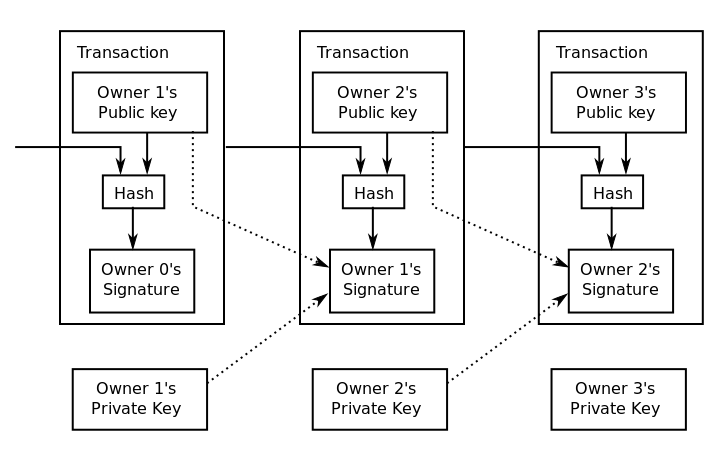
\includegraphics[scale=0.5]{images/transaction.png}

Looking at the transaction message more carefully, we see that Owner1 uses his private key to sign the transaction and generate a hash which he then passes on to Owner2. Owner2 then uses his public key to verify the ownership of the transaction. Thus, a chain of ownership for each bitcoin is maintained. By this process, we have ensured that transactions can be verified and validated without the need for a central authority. If a private key is lost, all the bitcoins associated with that key is also lost and cannot be recovered. There is a case of a man of a man losing his harddrive contatining his private key and thereby losing \$7.5 Million worth of bitcoins \cite{throw}. 

\section{Bitcoin Mining}
A bitcoin transaction on the network does not get added to the block chain (which contains accepted transactions) until it is verified and included in a block by a process called "mining". In order to motivate peers to validate transactions, new bitcoins are issued to them as a reward. Mining serves two main purposes:

\begin{enumerate}
\item Mining creates new bitcoins. This is similar to minting money in the real world.
\item It helps to verify the transactions involving bitcoins
\end{enumerate}

\section{Problem of Double Spending}
What happens if Alice has a bitcoin and tries to double spend with it with two people at the same time? Lets say Alice controls two machines that immediately verify and publish her two transactions to the block chain. Once published, they cannot be reversed. So how do we solve this problem?

This problem can be solved by using a concept known as proof of work. This concept relies on two main ideas:
\begin{enumerate}
\item Make it computationally costly to verify transactions in a block.
\item Reward people for validating the transactions.
\end{enumerate}

The benefit of making it costly to validate transactions now means that validation does not depend on the amount of network identities that a person has but depends on the amount of computational power that he has. With a small modification, we can make it such that a cheater would need enormous computing power to validate her transactions thus making it impractical. \\*

Suppose a miner has to validate Block B that contains a list of transactions t. He has to find a nonce (a number) and append it to the list of transactions t. When this is passed to the SHA-256 hash function and hashed, the output should begin with a large number of zeroes. The difficulty of the puzzle can be altered by requiring a larger number of trailing zeros. What makes this so difficult is that if the input changes even a little, the output from the hash function changes completely. So, if we want 10 trailing zeroes before our hash, we will have to try $16^{10} \approx 10^{12}$ different combinations before producing the correct nonce. \\*

Under this scenario, let us look at the issue of double spending again where Alice is trying to double spend her bitcoin. She sends one of her transactions to one set of miners and the other to another set of miners hoping to get both of them validated simultaneously. Lets call it Block A and Block B (containing Alice’s transactions). The miners who received Block A first will continue working on it while miners who received Block B will work on validating it. This creates a fork in the block chain. \\*
\begin{center}
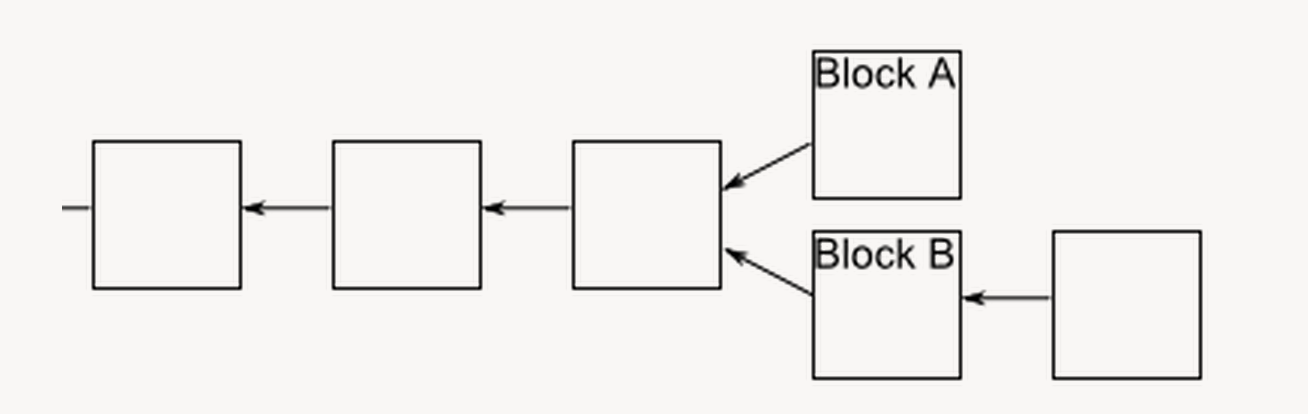
\includegraphics[scale=0.5]{images/fork.png}
\end{center}

Now, suppose miners working on fork B mine a block first. As soon as miners working on fork A hear this news, they will immediately abandon work on fork A and switch to fork B. So, the fork A will be abandoned at it can be ignored. In this way, only one of Alice’s transactions will be accepted. In real life, a transaction in Bitcoin is not considered accepted until:

\begin{enumerate}
\item It is part of the longest fork.
\item At Least 5 blocks follow it in the longest fork.
\end{enumerate}

Under these conditions, unless Alice is able to solve the proof-of-work as fast as everyone else (controlling fifty percent of the network’s computing power), one of the fork will become shorter and get abandoned. Thus double spending is avoided in the Bitcoin protocol.